Los procesos tecnicos que guiaron el diseño y desarrollo del sistema Thary se estructuraron siguiendo la ISO/IEC/IEEE 12207, una norma que establece un conjunto de procesos estandar para el ciclo de vida del software. Dichos procesos fueron aplicados al desarrollo del sistema de la siguiente manera:

\subsubsection{Identificación de Stakeholders}
A partir del planteamiento del sistema y tras un analisis de sus caracteristicas y funcionalidades, se identificaron los siguientes stakeholders que estaria involucrados en el sistema, ya sea directa o indirectamente:

\begin{itemize}
    \item Personal encargado de la gestion del inventario y el abastecimiento: Es el usuario final que interactua con el sistema, es responsable de interpretar los resultados que Thary y tomar decisiones de repocision en base a ellas.
    \item Equipo de desarrollo: Desarrolladores y diseñadores responsables de la implementación del sistema Thary, asegurando que cumpla con los requisitos y estándares establecidos.
    \item Administradores del sistema: Es el perfil con permisos y privilegios, es responsable de cargar los datos historicos de consumo, es decir, el archivo de entrada, ejecutar el proceso de prediccion, ademas, puede crear nuevos usaurios para los empleados con menor rango.
    \item Institucion usuaria del sistema: Es la entidad interesada en utilizar Thary para poder refucir el riesgo de desabastecimiento de productos. El sistema se planeo para poder adaptarse en distintos dominios, por lo que cualquier tipo de empresa puede usarlo.
    \item Proovedores de productos: Aunque los proovedores no interactuan con Thary, indirectamente son una variable importante para el sistema, ya que factores externos como el tiempo de entrega o lead time, marcan una gran diferencia en los resultados del sistema.
\end{itemize} 

\begin{table}[H]
\centering
\caption{Análisis de interés e influencia de los stakeholders}
\label{tab:stakeholders_interes_influencia}

\begin{tabularx}{\textwidth}{
    >{\raggedright\arraybackslash}p{4cm}
    >{\raggedright\arraybackslash}X
    >{\centering\arraybackslash}p{3cm}
    >{\centering\arraybackslash}p{3cm}
}
\hline
\textbf{Stakeholder} & \textbf{Interés} & \textbf{Influencia} \\
\hline

Personal de inventario y abastecimiento
& Alto
& Alta
\\

Administrador del sistema
& Alto
& Alta
\\

Institución usuaria
& Alto
& Alta
\\

Proveedores de productos
& Medio
& Media
\\

Equipo de desarrollo
& Alto
& Alta
\\

\hline
\end{tabularx}
\end{table}

\subsubsection{Elicitación de Requisitos}
La elicitacion de requisitos consiste en poder identificar las necesidades del sistema a partir de los usaurios, en el caso de Thary, el proceso se llevo a cabo mediante dos fuentes principales de informacion, en primera instancia, la revision de literatura permitio analizar que variables suelen ser relevantes para este tipo de proyectos, y que salidas le aportan mayor valor al usuario. En segundo lugar, se realizo un analisis a un caso de estudio real, los datos usados durante el desarrollo del sistema eran datos autenticos de la Clinica Nuestra señora de los Remedios de la ciudad de Cali, lo cual permitio observar como se comportaria el sistema en un escenario real como la existencia de variaciones en la demanda o datos historicos no tan limpios como historiales incompletos o datos con errores, y que ajustes serian necesarios para mejorar su rendimiento.

Es en base a tdo esto, que se definieron los siguientes requisitos funcionales:

\begin{itemize}
    \item RF-01: El sistema debe permitir que un usuario registrado como admin pueda realizar la carga de un archivo CSV con el datos como el historial de consumo mensual de los productos, validando que contenga los datos minimos requeridos: fecha, id del producto y cantidad demandada.
    \item RF-02: El sistema debe generar una estimacion de la demanda mensual, esperada para cada producto a partir de la informacion compartida en el historial cargado
    \item RF-03: El sistema debe de calcular para cada producto datos como el punto de reposicion y la cantidad recomendada de compra, considerando factores externos como el tiempo de entrega del proovedor o lead time, presupuestos y el inventario actual disponible
    \item RF-04: El sistema debe de contar con alertas visuales claras para los productos cuyo inventario actual se encuentre en o por debajo de su punto de reposicion.
    \item RF-05: El sistema debe presentar los resultados, demanda pronosticada, estado del inventario, etc, de una manera clara y sencilla de entender en una interfaz intuitiva para el usuario
    \item RF-06: El sistema debe permitirle al personal del inventario registrar un pedido, guardando informacion importante de este como proovedor elegido, fecha del pedido y el usuario responsable de la realizacion del pedido.
    \item RF-07: El sistema debe restringir el acceso a la carga de los archivos y la ejecucion del proceso unicamente al perfil administrador.
    \item RF-08: El sistema debe permitirle al perfil de administrador el poder crear nuevos usuarios con menos privilegios para sus empleados.
    \item RF-09: El sistema debe de permitir evaluar el desempeño de los modelos de prediccion mediante metricas cuantitavias, para de esta manera, poder respaldar la confiabilidad de las estimaciones que le son presentadas al usuario.
    \item RF-10: El sistema debe permitir el registro e inicio de sesion de los usuarios.
\end{itemize}

En cuanto a los requisitos no funcionales de Thary, se identificaron los siguientes:

\begin{itemize}
    \item RNF-01: Si el sistema es utilizado por mas de una organizacionm los datos de una no deben de ser accesibles para otra
    \item RNF-02: El sistema debe de poder procesar archivos de distintos dominios de inventario (salud, alimentos, ferreteria, etc) siempre y cuando contengan los datos minimos requeridos.
    \item RNF-03: El sistema debe poder generar una estimacion incluso si el historial de producto presenta datos faltantes.
\end{itemize}

\subsubsection{Especificación de Requisitos de Software (SRS)}

A partir de los requisitos especificados, se elaboro la especificacion de requisitos funcionales (SRP), la cual fue estructurada mediante casos de uso y tomando como referencia los lineamientos de la norma IEEE 29148 para la elaboracion de los mismos. El sistema contempla dos actores principales, el administrados y el personal de inventario. El administrador es el tipo de usuario que mas privilegios tiene, es responsable de cargar el historial de consumo e iniciar el procesamiento y gestionar las cuentas de los usuarios. Mientras que el personal de inventario solo usa el sistema para consultar las predicciones y, entre otras actividades, gestionar los pedidos sugeridos. La figura debajo representa el diagrama general de caso de uso de Thary:

\begin{figure}[H]
    \centering
    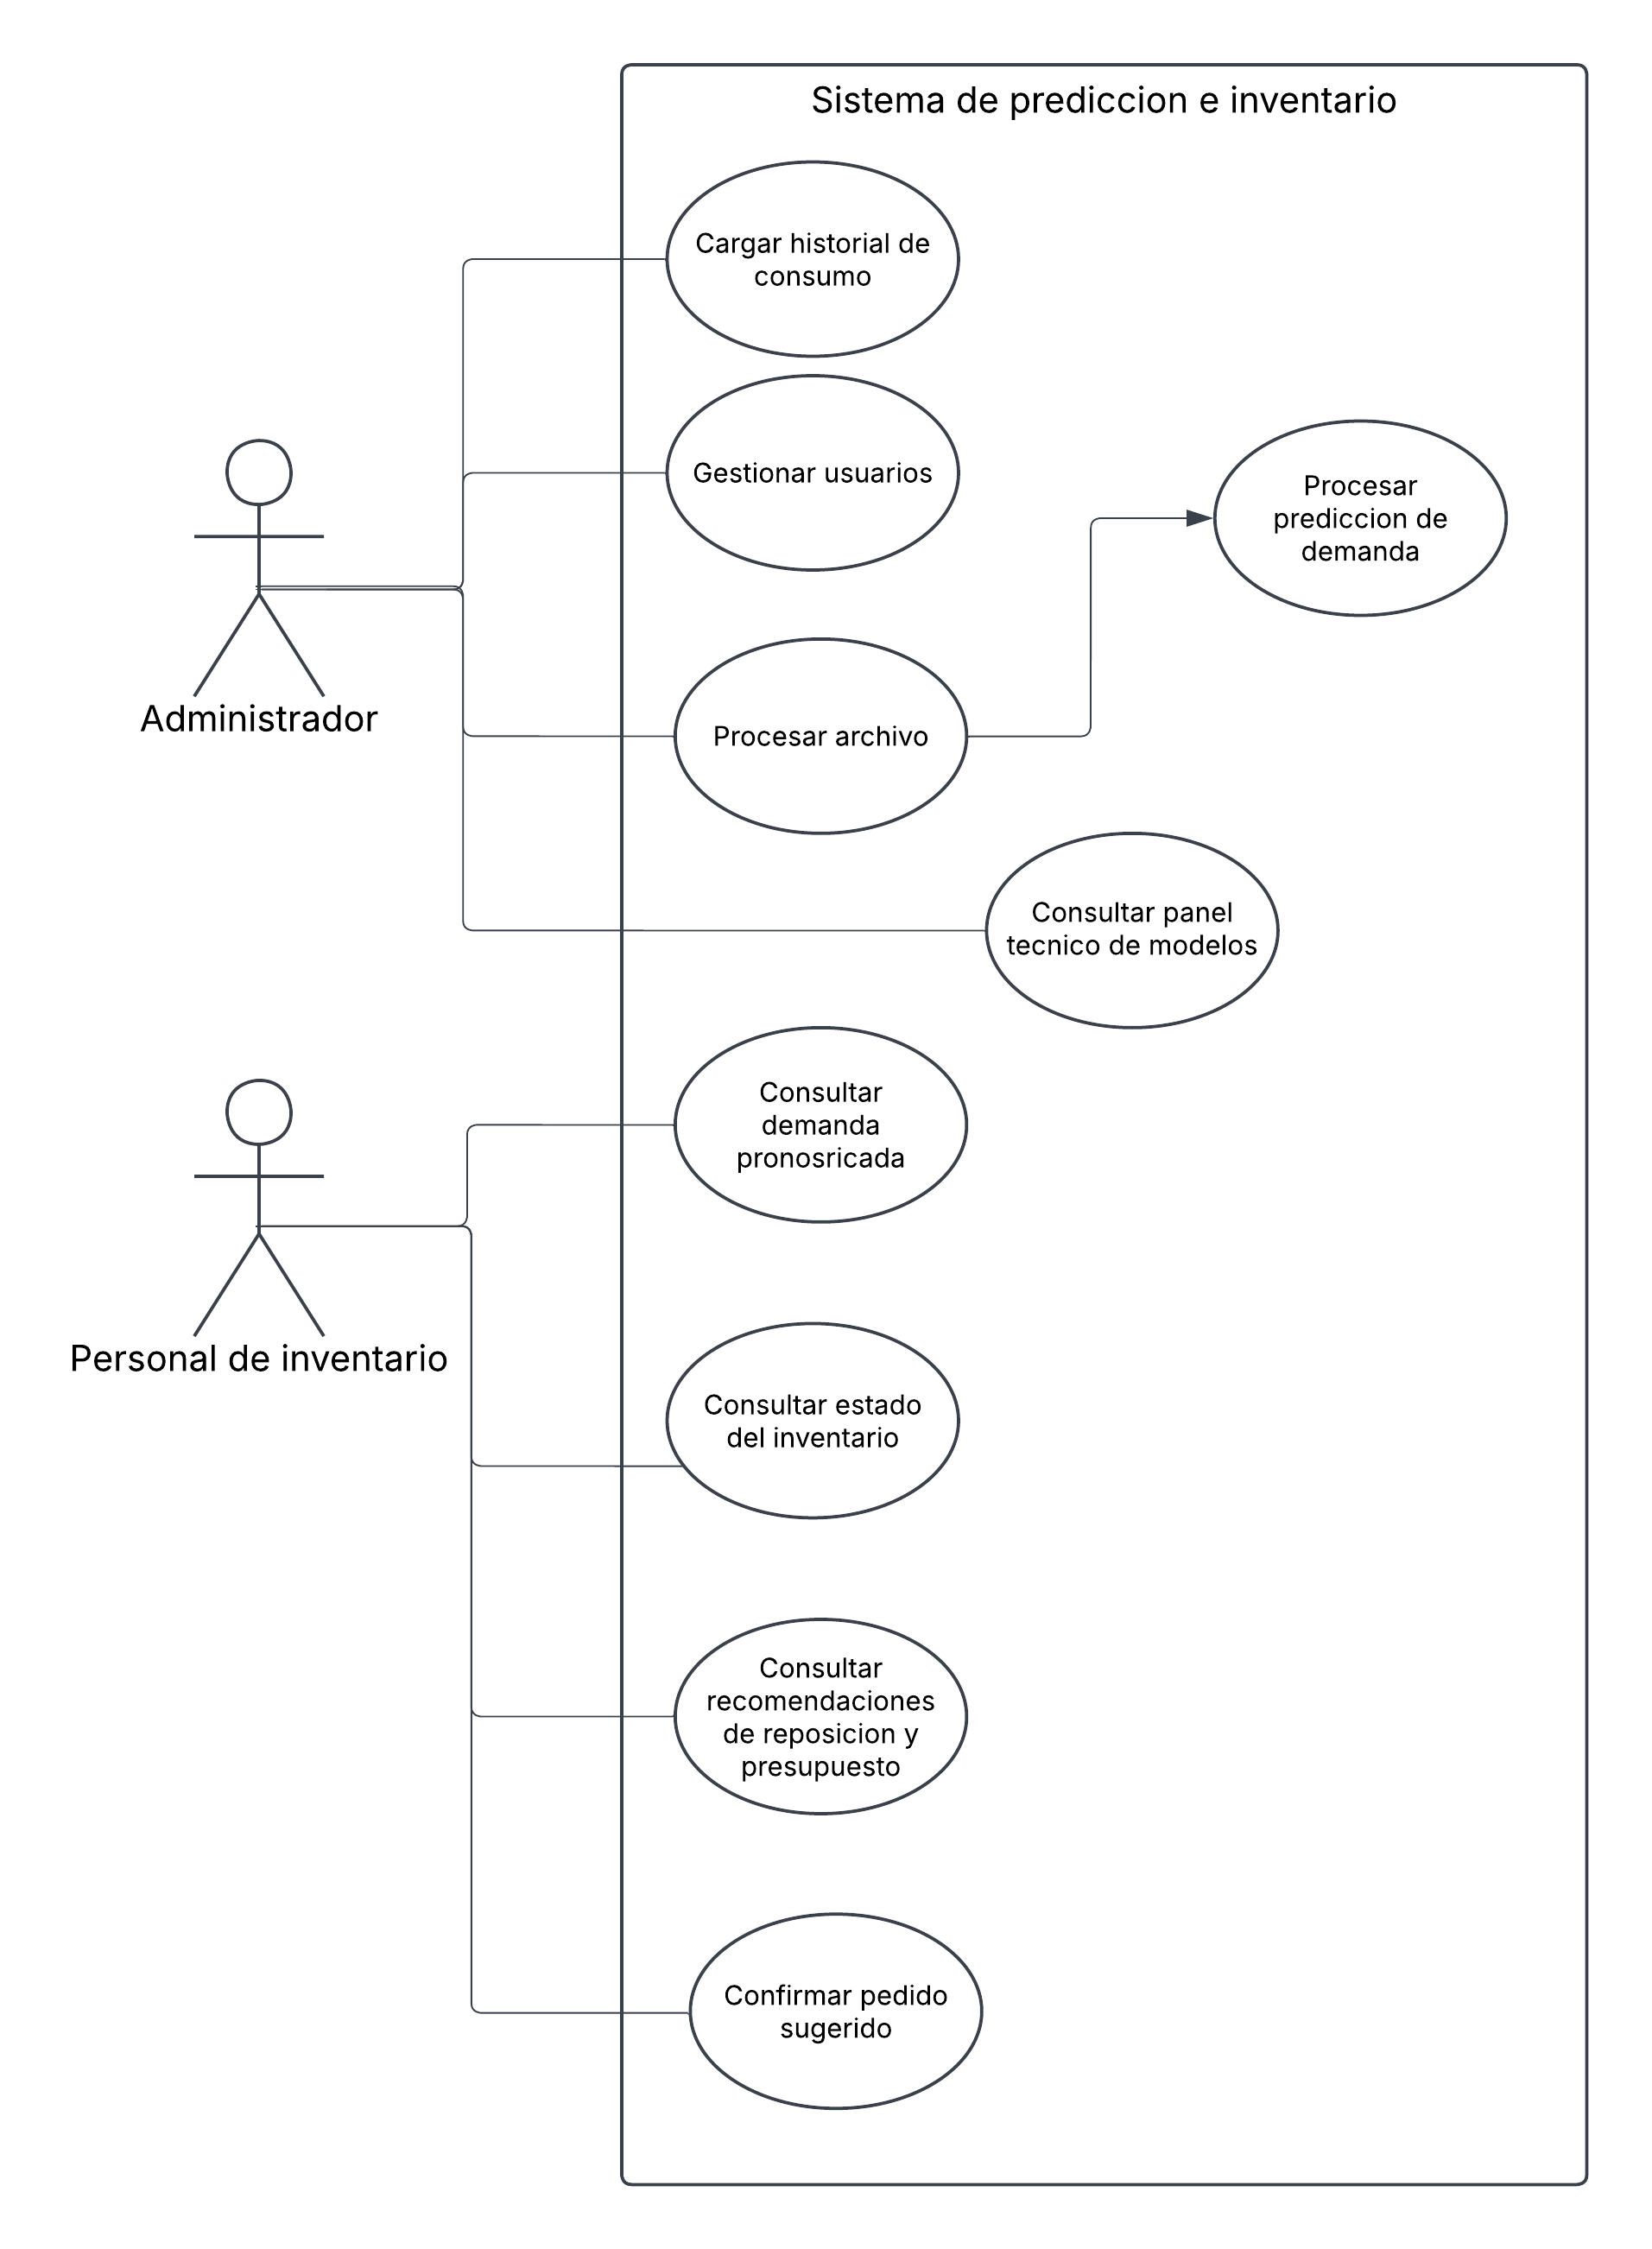
\includegraphics[width=1.0\textwidth]{templatefigures/caso_de_uso.png}
    \caption{Caso de uso}
\end{figure}

Como se puede ver en el diagrama, los casos de uso identificados, se relacionan con los requisitos funcionales de la siguiente manera:

\begin{table}[H]
\centering
\caption{Trazabilidad entre casos de uso y requisitos funcionales}
\label{tab:trazabilidad_casos_uso}
\begin{tabularx}{\textwidth}{>{\centering\arraybackslash}p{1.2cm} >{\raggedright\arraybackslash}X >{\raggedright\arraybackslash}X >{\centering\arraybackslash}p{3cm}}
\hline
\textbf{ID} & \textbf{Caso de uso} & \textbf{Actor principal} & \textbf{Requisitos relacionados} \\
\hline

CU-01 & Iniciar sesión & Usuario registrado & RF-10 \\

CU-02 & Cargar historial de consumo & Administrador & RF-01, RF-07 \\

CU-03 & Procesar archivo & Administrador & RF-02, RF-07 \\

CU-04 & Consultar demanda pronosticada & Personal de Inventario & RF-02, RF-05 \\

CU-05 & Consultar estado del inventario & Personal de Inventario & RF-04, RF-05 \\

CU-06 & Consultar recomendaciones de reposición y presupuesto & Personal de Inventario & RF-03, RF-05 \\

CU-07 & Registrar pedido & Personal de Inventario & RF-06 \\

CU-08 & Gestionar usuarios & Administrador & RF-08 \\

\hline
\end{tabularx}
\end{table}

\begin{itemize}

    \item Caso de uso CU-01 (Iniciar sesión (Usuario registrado)): Este caso de uso corresponde al RF-10, y le permite a cualquier usuario registrado ingresar al sistema mediante sus credenciales para acceder a las funcionalidades según su rol.

    \item Caso de uso CU-02 (Cargar historial de consumo (administrador)): Este caso de uso corresponde al RF-01, y permite al administrador seleccionar y cargar el archivo csv con el historial de consumo.

    \item Caso de uso CU-03 (Iniciar procesamiento(Administrador)): Corresponde al requerimiento RF-02, que hace referncia a que una vez cargado el archivo, el administrador debe de seleccionar la opcion "Procesar archivo" para que el sistema inicialice el procesamiento de los datos. 

    \item Caso de uso CU-04 (Consultar demanda pronosticada (Personal de inventario)): Este caso de uso corresponde al RF-02 y al RF-05, y le permite al usuario consultar la demanda mensual estimada para cada producto una vez el archivo ya ha sido procesado.

    \item Caso de uso CU-05 (Consultar estado del inventario (Personal de inventario)): Este caso de uso corresponde a RF-04, que permite al usuario visualizar tanto el inventario disponible como los productos que presentan condiciones de alerta.

    \item Caso de uso CU-06 (Consultar las recomendaciones de reposicion y presupuesto (Personal del inventario)): Corresponde al requisito RF-03, y le permite al usuario consultar las recomendaciones generadas por el sistema y la informacion asociada al presupuesto disponible

    \item Caso de uso CU-07 (Confirmar pedido (Personal de inventario)): Este se relaciona directamente con el RF-06, y permite marcar como completado las recomendaciones de pedido generadas por Thary. Los pedidos confirmados quedan registrados con el nombre de la persona que los completa.
    \item Caso de uso CU-08 (Gestionar cuentas de usuario(administrador)): Le permite al administrador el poder crear nuevas cuentas al personal del inventario

\end{itemize}

Todos los casos de uso se documentan individualmente en la especificacion SRS presentada en el Anexo A, la cual contempla detalles como objetivo, actor principal, precondiciones y postcondiciones, flujo principales y alternativos.

Elementos como las precondiciones se establecen antes de iniciar una funcionalidad, mientras que las postcondiciones describen cual es el estado esperado del sistema al finalizar el proceso, es de esta manera que realizar una correcta especificacion de casos permite establecer una base a la hora de continuar con el proceso de diseño de arquitectura e implementacion de servicios.

\subsubsection{Diseño de la Arquitectura}

El sistema Thary fue diseñado basandose en una organizacion pipeline para el componente de prediccion y un estilo arquitectonico en capas de las cuales se distinguen tres principales:

\begin{itemize}
    \item Capa de Presentacion: Esta capa es la reponsable de funcionalidades como carga de archivos, visualizacion de resultados, registro de pedidos y demas funcionalidades relacionadas con toda la interaccion que el usuario final va a tener con el sistema.
    \item Capa de Control: Esta capa es la encargada de recibir todas las solicitudes que el usaurio le haga a la aplicacion, y devolver los resultados esperados a la capa de presentacion
    \item Capa de servicios de dominio: En esta capa se encuentra el componente de prediccion organizado como un pipeline secuencial compuesto por las diferentes etapas del sistema, en general, en esta capa se concentra toda la logica de Thary. 
\end{itemize}

En cuanto a porque se decidio llevar la organizacion mediante un pipeline, esta desicion se tomo debido a que el proceso de prediccion de demanda, por su naturaleza, corresponde a un flujo secuencial de transformacion de los datos, por lo que el uso de esta estructuta facilita que se pueda separar responsabilidades de una manera mas sencilla y la trazabilidad de los resultados obtenidos. 

Por otro lado, a la hora de elegir como se manejaria la persistencia de la informacion, se opto por simplemente utilizar archivos estructurados, en lugar de utilizar algun motor de base de dato relacional. Esta desicion se tomo considerando el alcance del proyecto y de esta manera, evitando involucrar complejidad adicional al mismo. Aun asi, la arquitectura de Thary contempla el aislamiento de los datos para cada organizacion, de manera que todas cuentan con un espcio independiente evitando que puedan acceder a informacion de otro usuario. 

\paragraph{Escenarios Arquitecturales}
% Guia: escenarios de calidad (rendimiento, disponibilidad, seguridad) que
% guian la arquitectura.
Para garantizar que Thary cuenta con una arquitectura que es capaz de responder a los atributos de calidad necesarios para un proyecto con sus caracteristicas, se plantaron los siguientes escenarios:
\begin{itemize}
    \item Escenario 1 (Confiabilidad ante datos escasos): Este escenario hace referencia a que cuando un usuario carge el historial de un producto con menos de cuatro meses de registros, Thary no debe de fallar ni excluir el producto, en su lugar, debe de utilizar un metodo de estimacion de respaldo, como la media movil. Esto le aporta valor al sistema cuando no exista suficiente informacion historica para usar un modelo mas complejo.
    \item Escenario 2 (Desempeño ante catologos extensos): Los calculos de variables como puntos de reposicion y cantidaddes sugeridas, deben de poder completarse de manera eficiente sin importar si cuando se proceso el archivo con los datos, este contiene un numero alto de diferntes productos. 
    \item Escenario 3 (Confidencialidad de la informcion): En este escenario se tiene en cuenta que Thary debe garantizar que los datos relacionados con el inventario y el historial de consumo de la organizacion, no se transmitan a ningun servicio externo del que Thary se encuentra alojado.
    \item Escenario 4 (Aislamiento entre organizaciones): Al trabajar con tantos usuarios/administradoes, lo mas probable es que en algun moemtno, al menos dos organizaciones distintar usen el sistema de manera simultane, Thary debe asegurarse que ningun tipo de dato quede expuesto ni pueda ser modificado por otra organizacion 
    \item Escenario 5 (Adaptabilidad del formato de datos): Este escenario se refiere a que cuando se cargue un archivo que pertenezca a un dominio diferente al caso de estudio principal, el cual fue salud, Thary tiene que ser capaz de reconocer y normalizar las columnas sin tener que modificar el codigo.
\end{itemize}

Estos escenarios permiten poder verificar que las desiciones arquitectonicas tomadas respondan a las necesidades que tiene el sistema, facilitando que posteriormente se pueda comprobar el funcionamiento de Thary
\paragraph{Análisis de Alternativas y Decisiones de Diseño (ADRs)}
% Guia: alternativas evaluadas y decisiones de arquitectura (ADR):
% contexto, decision, consecuencias.

Las decisiones de diseño que fueron adoptadas durante todo el desarrollo del sistema Thary y las alternativas consideradas.

\begin{itemize}
     \item Decision 1 (Persistencia basada en archivos frente a base de datos relacional): 
     \item
\end{itemize}
        
\paragraph{Representación de la Arquitectura (Modelo C4)}
% Guia: diagramas C4: contexto, contenedores, componentes y (si aplica) codigo.

% ---------------------------------------------------------------------
% EJEMPLO DE FIGURA (borrelo y ponga la suya)
%   - guarde su imagen en la carpeta images/
%   - \includegraphics[width=...]{nombre-del-archivo}  (sin la extension)
%   - el \label debe ir DESPUES del \caption
%   - se referencia en el texto con \ref{fig:c4-contexto}
% ---------------------------------------------------------------------
\begin{figure}[H]
    \centering
    \includegraphics[width=0.7\textwidth]{example-image}
    \caption{Diagrama de contexto del sistema (nivel 1 del modelo C4).}
    \label{fig:c4-contexto}
\end{figure}

Como se observa en la Fig. \ref{fig:c4-contexto}, el sistema interactúa con los
actores identificados en la sección \ref{sec:stakeholders}.


\subsubsection{Diseño Detallado}


\paragraph{Modelo de Datos}
% Guia: modelo conceptual, logico y fisico.
% El diccionario de datos va en el Anexo B.

% ---------------------------------------------------------------------
% EJEMPLO DE TABLA (borrela y ponga la suya)
%   - en esta plantilla el rotulo va ENCIMA de la tabla
%   - la columna X reparte el ancho sobrante automaticamente
%   - se referencia en el texto con \ref{tab:entidades}
% ---------------------------------------------------------------------
\begin{table}[H]
    \centering
    \caption{Entidades principales del modelo de datos.}
    \label{tab:entidades}
    \begin{tabularx}{\textwidth}{lXl}
        \toprule
        \textbf{Entidad} & \textbf{Descripción} & \textbf{Cardinalidad} \\
        \midrule
        Usuario   & Persona registrada en el sistema.   & 1 : N \\
        Proyecto  & Trabajo gestionado por un usuario.  & 1 : N \\
        Actividad & Tarea que pertenece a un proyecto.  & N : 1 \\
        \bottomrule
    \end{tabularx}
\end{table}

La Tabla \ref{tab:entidades} resume las entidades del modelo.


\paragraph{Diseño UX/UI}
% Guia: flujos de usuario, wireframes y criterios de usabilidad y accesibilidad.


\subsubsection{Análisis de Amenazas y Diseño Seguro}
% Guia: modelado de amenazas (STRIDE u otro) y controles de diseno seguro.


\subsection{Construcción, Integración y Despliegue}
% Guia: practicas de codificacion, control de versiones, CI/CD y ambientes
% de despliegue.

% ---------------------------------------------------------------------
% EJEMPLO DE CODIGO FUENTE (borrelo)
%   el lenguaje va entre llaves: {python}, {java}, {sql}, {bash}, ...
%   Lo compone el paquete listings. Para colorearlo con minted, active el
%   interruptor que hay en template/packages.tex.
% ---------------------------------------------------------------------
\begin{minted}{python}
def calcular_cobertura(lineas_probadas, lineas_totales):
    # Devuelve el porcentaje de cobertura de pruebas
    if lineas_totales == 0:
        return 0.0
    return 100.0 * lineas_probadas / lineas_totales
\end{minted}


\subsection{Plan de Verificación y Validación}
% Guia: estrategia de pruebas, criterios de aceptacion y plan de validacion
% con usuarios.
